\documentclass[a4paper]{article}
\usepackage[utf8]{inputenc}
\usepackage[spanish, es-tabla]{babel}
\usepackage[table,xcdraw]{xcolor}
\usepackage{amsmath}
\usepackage{amsfonts}
\usepackage{amssymb}

\usepackage{float}
\usepackage{graphicx}

\usepackage{caption}
\usepackage{subcaption}
\captionsetup{compatibility=false}

\usepackage{multirow}
\setlength{\doublerulesep}{\arrayrulewidth}

\newcommand{\quotes}[1]{``#1''}
\newcommand\underrel[2]{\mathrel{\mathop{#2}\limits_{#1}}}

\usepackage{array}
\newcolumntype{C}[1]{>{\centering\let\newline\\\arraybackslash\hspace{0pt}}m{#1}}

\usepackage[american]{circuitikz}
\usepackage{xcolor}
\usepackage{fancyhdr}

\newlength{\stockheight}
\usepackage{hyperref}

\hypersetup{
    colorlinks=true,
    linkcolor=blue,
    filecolor=magenta,      
    urlcolor=blue,
    citecolor=blue,    
}

\urlstyle{same}

\usepackage{units} 
\pagestyle{fancy}
\fancyhf{}

\rfoot{Página \thepage}



\begin{document}
\subsection{Introducción}
En esta sección se implementó una compuerta \textbf{NOT} utilizando diversas tecnologías, siendo estas TTL (Transistor-Transistor-Logic), RTL (Resistor-Transistor-Logic) mediante transistores BJT (Bipolar Junction Transistor) y finalmente una variación de RTL utilizando un transistor MOSFET (Metal Oxide Semiconductor Field Efect Transistor).
\subsection{Comparación tecnologías.}
Usaremos dos tipos de transistores, siendo estos BJT y MOSFET.
\begin{itemize}
\item Los BJT son controlados por corriente, mientras que los MOS son controlados por tensión.
\item Los BJT tienen una respuesta mas veloz ante un cambio en su modo de funcionamiento\footnote{Satuación y corte} que los MOS dado a que poseen una menor capacidad.
\item Los transistores MOS tienen una mayor estabilidad frente a la temperatura que los BJT.	
\item Los transistores BJT cuentan con una corriente de polarización de base que los MOS no tienen ($I_g =0$).
\item La impedancia de entrada de los MOS es mucho mayor que la de los BJT.
\end{itemize}
\subsection{Circuitos Propuestos.}
Los circuitos propuestos son los siguientes:

\begin{figure}[H]	
	\centering
	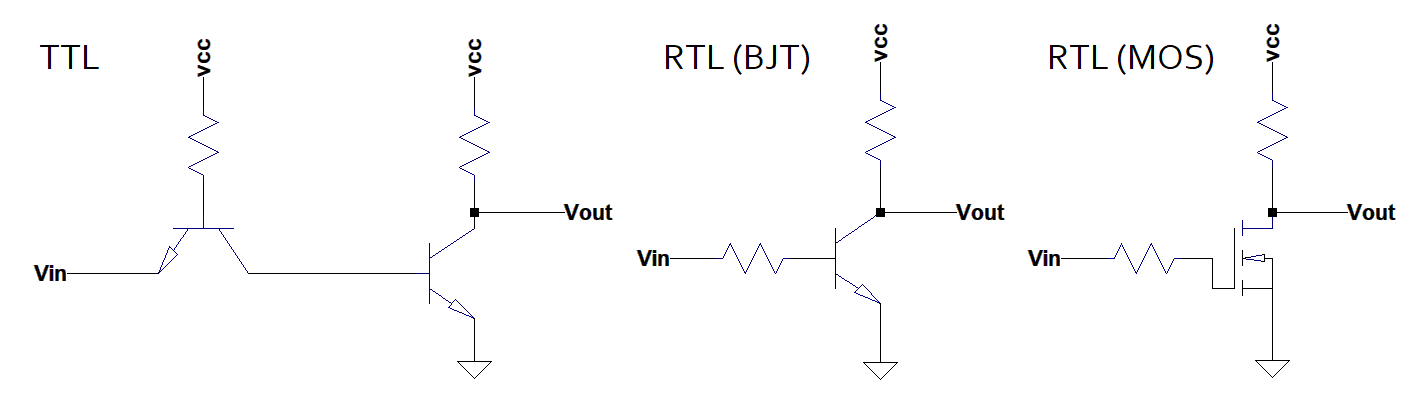
\includegraphics[width=\textwidth]{Imagenes/CircuitosPropuestos.PNG}
	\caption{Circuitos Propuestos.}
	\label{fig:circprop}
\end{figure}

\subsection{Diseño PCB.}
Se implementó en un único PCB los 3 circuitos, que corresponden al siguiente esquemático:
\begin{figure}[H]	
	\centering
	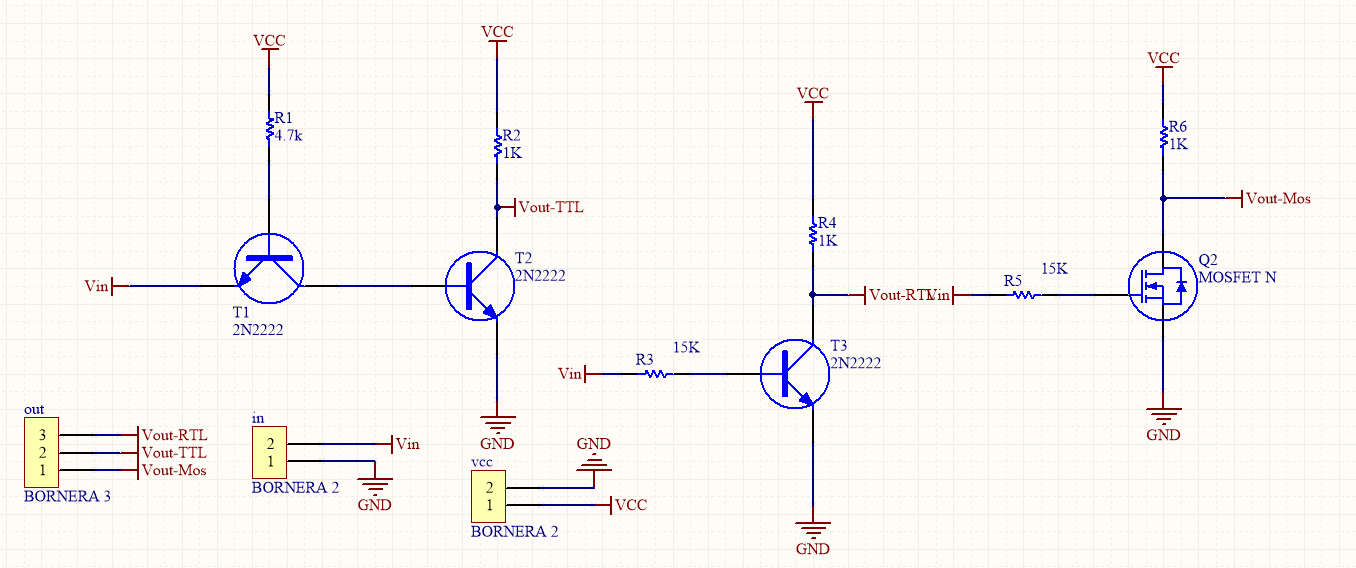
\includegraphics[width=\textwidth]{Imagenes/Esquematico.PNG}
	\caption{Esquemático.}
	\label{fig:esquematico}
\end{figure}
\begin{figure}[H]	
	\centering
	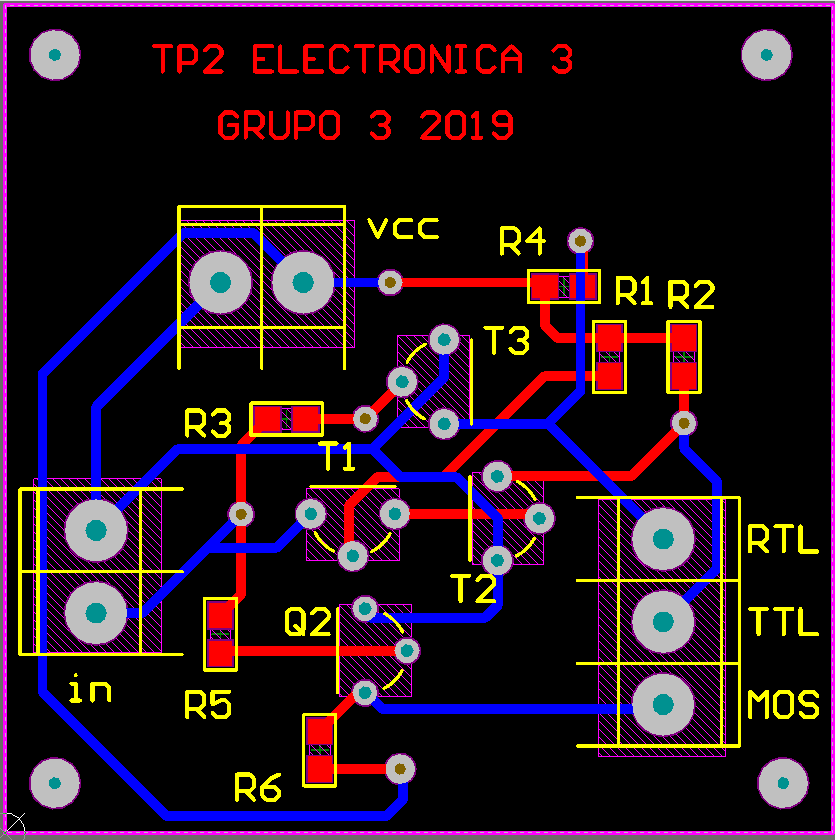
\includegraphics[width=0.5\textwidth]{Imagenes/PCB.PNG}
	\caption{PCB.}
	\label{fig:pcb}
\end{figure}

\subsection{Observables de interés.}
\label{sec:Obs}
Se seleccionaron como observables de interés los siguientes parámetros:
\begin{itemize}
\item High-level input voltage
\item Low-level input voltage
\item High-level output voltage
\item Low-level output voltage
\item Noise Margin
\item Popagation delay High to Low
\item Popagation delay Low to High
\item Transition delay High to Low
\item Transition delay Low to High
\item Maximum output current
\end{itemize}
\subsection{Análisis de resultados.}
Para realizar una comparación entre los modelos propuestos, se utilizarán los observables de interés definidos en la sección (\ref{sec:Obs}) utlizando la siguiente tabla:


\end{document}
